% ============================================================
% 2020 高教社杯全国大学生数学建模竞赛
% A题：炉温曲线建模与优化
% ============================================================
\documentclass[12pt,a4paper]{ctexart}

% ---------- 页面设置 ----------
\usepackage[top=2.5cm, bottom=2.5cm, left=2.5cm, right=2.5cm]{geometry}
\usepackage{amsmath,amssymb}
\usepackage{graphicx}
\usepackage{booktabs}
\usepackage{tabularx}
\usepackage{caption}
\usepackage{hyperref}
\usepackage{enumitem}
\usepackage{float}
\usepackage{fancyhdr}
\setlength{\headheight}{14pt}
\usepackage{xcolor}
\usepackage{listings}
\lstset{
    basicstyle=\small\ttfamily,
    numbers=left,
    numberstyle=\tiny\color{gray},
    frame=single,
    backgroundcolor=\color{gray!10},
    rulecolor=\color{gray!50},
    breaklines=true,
    breakatwhitespace=false,
    xleftmargin=1em,
    xrightmargin=1em,
    language=Matlab,
    keywordstyle=\color{blue},
    commentstyle=\color{green!50!black},
    stringstyle=\color{red},
}

% 表格满宽命令
\newcolumntype{Y}{>{\centering\arraybackslash}X}

\hypersetup{colorlinks=true, linkcolor=black, citecolor=black, urlcolor=black}
\captionsetup{font=small, labelfont=bf}
\setlength{\emergencystretch}{1em}

% 参考文献上标
\makeatletter
\def\@cite#1{\textsuperscript{[#1]}}
\makeatother

% ---------- 页眉页脚 ----------
\pagestyle{fancy}
\fancyhf{}
\fancyfoot[C]{\thepage}
\renewcommand{\headrulewidth}{0pt}

% ---------- 标题信息 ----------
\title{\vspace{-2cm}\textbf{回焊炉炉温曲线建模与优化}}
\author{}
\date{}

\begin{document}

\maketitle
\thispagestyle{empty}

% ============================================================
\section*{摘\quad 要}
\thispagestyle{fancy}
% ============================================================

回焊炉是印刷电路板（PCB）焊接工艺中的核心设备，其炉温曲线的精确控制对焊接质量至关重要。
本文围绕回焊炉焊接区域的温度变化规律与工艺参数优化问题，建立了一维非稳态热传导模型，通过数值模拟与全局优化方法对炉温曲线进行建模与求解。

针对\textbf{问题1}，建立了基于一维非稳态热传导偏微分方程的机理模型，采用Crank--Nicolson隐式有限差分格式进行数值求解。
通过SelPSO（带自然选择的粒子群优化算法）对附件实验数据独立拟合，获得了5段分区热力学参数（拟合优度$R^2=0.9999$，均方根误差$\mathrm{RMSE}=0.62^{\circ}\mathrm{C}$）。
在给定传送带速度$v=78\;\mathrm{cm/min}$和各温区设定温度的条件下，计算得到焊接区域中心峰值温度为$240.6^{\circ}\mathrm{C}$，
小温区3中点、6中点、7中点及小温区8结束处的温度分别为$129.5^{\circ}\mathrm{C}$、$167.9^{\circ}\mathrm{C}$、$189.9^{\circ}\mathrm{C}$和$223.8^{\circ}\mathrm{C}$，
每隔0.5秒的温度数据已保存至result.csv。

针对\textbf{问题2}，利用速度—温度指标的单调性，采用二分搜索确定满足制程界限的最大传送带速度。
在温区设定温度$T_{1-5}=182^{\circ}\mathrm{C},T_6=203^{\circ}\mathrm{C},T_7=237^{\circ}\mathrm{C},T_{8-9}=254^{\circ}\mathrm{C}$的条件下，
求得最大传送带速度为$\boldsymbol{80.83\;\mathrm{cm/min}}$，限制瓶颈为峰值温度不低于$240^{\circ}\mathrm{C}$的约束。

针对\textbf{问题3}，以超过$217^{\circ}\mathrm{C}$到峰值温度所围面积为最小化目标，采用SelPSO在5维决策空间中全局优化。
最优温区设定为$T_{1-5}=178.1^{\circ}\mathrm{C},T_6=194.3^{\circ}\mathrm{C},T_7=225.9^{\circ}\mathrm{C},T_{8-9}=265.0^{\circ}\mathrm{C}$，
传送带速度$v=90.90\;\mathrm{cm/min}$，最小面积$\boldsymbol{391.6\;^{\circ}\mathrm{C}\!\cdot\!\mathrm{s}}$。
在此参数下，峰值温度为$240.0^{\circ}\mathrm{C}$（恰好触及约束下界），$150\sim190^{\circ}\mathrm{C}$升温时间为$63.0\;\mathrm{s}$，温度大于$217^{\circ}\mathrm{C}$的时间为$54.5\;\mathrm{s}$。

针对\textbf{问题4}，构造了双维度综合对称性指标$\sigma=\max(\sigma_1,\sigma_2)$，其中$\sigma_1$衡量面积对称性，$\sigma_2$衡量时间对称性。
以$\sigma$为目标函数的SelPSO优化得到最优参数，对称性指标从问题3的$0.1833$改善至$\boldsymbol{0.1803}$，
面积从$391.6\;^{\circ}\mathrm{C}\!\cdot\!\mathrm{s}$增加至$408.8\;^{\circ}\mathrm{C}\!\cdot\!\mathrm{s}$，以$4.4\%$的面积代价换取了$1.6\%$的对称性改善。

\textbf{模型创新点}包括：(1)~基于回焊炉四大功能区域的5段分区热力学参数策略；
(2)~Crank--Nicolson矩阵预分解技术，避免了逐时间步的三对角方程求解，显著提升计算效率；
(3)~SelPSO全局优化在参数估计和工艺优化中的应用；
(4)~面积与时间双维度综合对称性指标的构造。
参数敏感性分析表明，模型对热力学参数$\pm10\%$的摄动具有良好鲁棒性（峰值温度偏移$<0.5^{\circ}\mathrm{C}$）。

\begin{flushright}
    \textbf{关键词}：炉温曲线；Crank--Nicolson有限差分；热传导方程；粒子群优化；对称性指标
\end{flushright}

\newpage

% ============================================================
\section{问题重述}
% ============================================================

\subsection{问题背景}

在集成电路板等电子产品生产中，印刷电路板（PCB）需放置在回焊炉中通过加热将电子元件自动焊接到电路板上。
回焊炉内部设有11个小温区，从功能上分为预热区、恒温区、回流区和冷却区四大区域。
各温区设定的温度及传送带过炉速度决定了焊接区域的温度变化（即炉温曲线），对产品质量至关重要。
目前，该领域的工艺参数调控主要依赖实验测试，缺乏系统的机理建模与优化方法。

某回焊炉内有11个小温区，每个小温区长度为30.5~cm，相邻小温区之间有5~cm的间隙，炉前区域和炉后区域长度均为25~cm。
焊接区域的厚度为0.15~mm，生产车间温度保持在$25^{\circ}\mathrm{C}$。
温度传感器在焊接区域中心温度达到$30^{\circ}\mathrm{C}$时开始工作。

\subsection{制程界限}

生产过程中，炉温曲线必须满足以下制程界限：
\begin{enumerate}[label=(\arabic*),nosep]
    \item 峰值温度：$240^{\circ}\mathrm{C} \leq T_{\max} \leq 250^{\circ}\mathrm{C}$；
    \item 温度上升过程中在$150^{\circ}\mathrm{C}\sim190^{\circ}\mathrm{C}$的时间：$60\;\mathrm{s} \leq t_{150-190} \leq 120\;\mathrm{s}$；
    \item 温度大于$217^{\circ}\mathrm{C}$的时间：$40\;\mathrm{s} \leq t_{>217} \leq 90\;\mathrm{s}$；
    \item 最大升/降温速率：$|dT/dt|_{\max} \leq 3\;^{\circ}\mathrm{C}/\mathrm{s}$。
\end{enumerate}

各小温区设定温度可在实验基准值基础上进行$\pm10^{\circ}\mathrm{C}$范围内的调整，传送带过炉速度调节范围为$65\sim100\;\mathrm{cm/min}$。

\subsection{需要解决的问题}

\begin{enumerate}[label=\textbf{问题\arabic*：},nosep,leftmargin=4.5em,labelsep=0.5em,itemindent=0pt]
    \item 建立焊接区域温度变化规律的数学模型。假设传送带过炉速度为78~cm/min，各温区设定温度为$173^{\circ}\mathrm{C}$（小温区1$\sim$5）、$198^{\circ}\mathrm{C}$（小温区6）、$230^{\circ}\mathrm{C}$（小温区7）和$257^{\circ}\mathrm{C}$（小温区8$\sim$9），给出焊接区域中心的温度变化情况，列出指定位置的温度，绘制炉温曲线，并将每隔0.5~s的温度数据保存到result.csv中。
    \item 假设各温区设定温度为$182^{\circ}\mathrm{C}$（小温区1$\sim$5）、$203^{\circ}\mathrm{C}$（小温区6）、$237^{\circ}\mathrm{C}$（小温区7）、$254^{\circ}\mathrm{C}$（小温区8$\sim$9），确定允许的最大传送带过炉速度。
    \item 在满足制程界限的前提下，以超过$217^{\circ}\mathrm{C}$到峰值温度所覆盖的面积最小为优化目标，确定最优炉温曲线及各温区的设定温度和传送带速度。
    \item 在问题3的基础上，进一步要求以峰值温度为中心线的两侧超过$217^{\circ}\mathrm{C}$的炉温曲线尽量对称，给出最优炉温曲线及相应的参数和指标值。
\end{enumerate}

% ============================================================
\section{模型假设}
% ============================================================

本文的模型假设分为三类：题目给定的条件假设、解题所必需的基础假设、以及为简化分析而引入的补充假设。

\subsection{题目给定条件假设}

\begin{enumerate}[label=\textbf{A\arabic*：},nosep]
    \item 回焊炉启动后炉内空气温度在短时间内达到稳定，各温区温度保持恒定；
    \item 生产车间温度保持在$25^{\circ}\mathrm{C}$；
    \item 传送带匀速运行，焊接区域位置满足$x=vt$；
    \item 小温区1$\sim$5温度保持一致，小温区8$\sim$9温度保持一致，小温区10$\sim$11固定为$25^{\circ}\mathrm{C}$。
\end{enumerate}

\subsection{解题基础假设}

\begin{enumerate}[label=\textbf{B\arabic*：},nosep]
    \item \textbf{一维传热假设}：焊接区域厚度（0.15~mm）远小于其长度和宽度（$<0.1\%$），仅考虑厚度方向的一维热传导；
    \item \textbf{对流换热边界}：电路板上下表面的换热服从牛顿冷却定律，忽略高温区的辐射传热效应；
    \item \textbf{分段常物性}：不同温度区域内电路板的热物理性质（热导率、比热容）视为常数，不同区域可取值不同。
\end{enumerate}

\subsection{补充假设}

\begin{enumerate}[label=\textbf{C\arabic*：},nosep]
    \item 炉前区域、炉后区域以及小温区之间的间隙不做特殊温度控制，其温度按相邻温区温度线性过渡；
    \item 忽略传送带速度波动和PCB位置偏差的影响。
\end{enumerate}

% ============================================================
\newpage
\section{符号说明}
% ============================================================

本文使用的主要符号及其含义见表\ref{tab:symbols}。

\begin{table}[H]
\centering
\caption{主要符号说明}
\label{tab:symbols}
\begin{tabular}{p{3.3cm}p{9.3cm}p{2.5cm}}
\toprule
\textbf{符号} & \textbf{含义} & \textbf{单位} \\
\midrule
$T(z,t)$   & 焊接区域温度分布 & $^{\circ}\mathrm{C}$ \\
$T_{air}(x)$ & 炉内环境温度分布 & $^{\circ}\mathrm{C}$ \\
$T_{1-5}$  & 小温区1$\sim$5设定温度（决策变量） & $^{\circ}\mathrm{C}$ \\
$T_{6}$    & 小温区6设定温度（决策变量） & $^{\circ}\mathrm{C}$ \\
$T_{7}$    & 小温区7设定温度（决策变量） & $^{\circ}\mathrm{C}$ \\
$T_{8-9}$  & 小温区8$\sim$9设定温度（决策变量） & $^{\circ}\mathrm{C}$ \\
$v$        & 传送带速度（决策变量） & cm/min \\
$a$        & 热扩散系数，$a=\sqrt{k/(\rho c)}$ & $\mathrm{cm}/\mathrm{s}^{1/2}$ \\
$h$        & 无量纲换热系数，$h=h_1/k$ & $\mathrm{cm}^{-1}$ \\
$l=0.015$  & 焊接区域厚度 & cm \\
$L=435.5$  & 回焊炉总长度 & cm \\
$T_{\max}$ & 峰值温度 & $^{\circ}\mathrm{C}$ \\
$S$        & 超过$217^{\circ}\mathrm{C}$到峰值的面积 & $^{\circ}\mathrm{C}\!\cdot\!\mathrm{s}$ \\
$\sigma$   & 综合对称性指标 & 无量纲 \\
\bottomrule
\end{tabular}
\end{table}

% ============================================================
\section{问题分析}
% ============================================================

\subsection{整体分析}

回焊炉焊接过程的炉温曲线建模涉及三个核心环节：
第一，\textbf{机理建模}——焊接区域内部的传热过程遵循热传导定律，炉内环境温度由各温区设定温度决定，需要建立连接两者的数学模型；
第二，\textbf{参数估计}——模型中的热力学参数（热扩散系数$a$和换热系数$h$）无法直接测量，需利用附件提供的实验数据通过反演优化确定；
第三，\textbf{数值求解}——偏微分方程需要稳定、高效的数值方法进行离散求解。

四个问题之间呈递进关系：问题1建立基础模型和求解器，为后续问题提供核心计算能力；
问题2利用单调性将约束满足问题转化为二分搜索；
问题3和问题4则是在约束条件或目标函数上的逐层扩展，从单目标面积最小化到带对称性要求的双目标优化。

\subsection{问题1分析}

问题1要求建立焊接区域温度变化的数学模型。由于PCB焊接区域厚度（0.15~mm）远小于其长度和宽度，可合理简化为一维非稳态热传导问题。
炉内环境温度由各温区设定温度按分段线性函数确定，焊接区域与环境之间通过对流换热进行热量交换。
建立偏微分方程后，采用Crank--Nicolson隐式有限差分格式进行数值求解，其具有二阶时间精度和无条件稳定性的优势。
模型中的热力学参数需要通过附件实验数据拟合确定。

\subsection{问题2分析}

传送带速度$v$与炉温曲线指标之间存在单调关系：速度越大，PCB在炉内停留时间越短，峰值温度越低，$>$$217^{\circ}\mathrm{C}$时间越短，同时温度变化斜率越大。
各指标中，最先触及约束边界的指标成为速度的限制瓶颈。
利用这一单调性，可将寻找最大可行速度的问题转化为二分搜索问题，在$[65,100]\;\mathrm{cm/min}$区间内高效收敛到边界值。

\subsection{问题3分析}

问题3要求最小化超过$217^{\circ}\mathrm{C}$到峰值温度的面积。决策变量为4个温区设定温度加传送带速度，共5维。
面积与各决策变量之间的关系高度非线性，需采用全局优化算法。
SelPSO（带自然选择的粒子群优化）通过模拟粒子群的社会行为搜索全局最优解，自然选择机制淘汰适应度差的粒子，有效避免陷入局部最优。

\subsection{问题4分析}

问题4在问题3的基础上增加对称性要求。对称性的度量涉及两个维度：峰值左右两侧面积的对称性和时间的对称性。
本文构造双维度综合对称性指标$\sigma=\max(\sigma_1,\sigma_2)$，其中$\sigma_1$为面积对称性，$\sigma_2$为时间对称性。
将该指标作为SelPSO的目标函数，在满足所有制程界限的约束下寻找对称性最优的工艺参数。

% ============================================================
\section{模型建立}
% ============================================================

\subsection{热传导控制方程}

焊接区域内部的温度场满足一维非稳态热传导方程\cite{ref1}：

\begin{equation}\label{eq:heat}
\frac{\partial T}{\partial t} = a^2 \frac{\partial^2 T}{\partial z^2}, \quad 0 < z < l, \quad t > 0
\end{equation}

其中$a^2 = k/(\rho c)$为热扩散系数，$k$为热导率，$\rho$为密度，$c$为比热容。

\textbf{初始条件}：$T(z,0)=25^{\circ}\mathrm{C}$（车间环境温度）。

\textbf{边界条件}：电路板上下表面服从牛顿冷却定律（对流换热）：

\begin{equation}\label{eq:bc}
-\left.\frac{\partial T}{\partial z}\right|_{z=0} = h[T_{air}(x) - T(0,t)],\qquad
\left.\frac{\partial T}{\partial z}\right|_{z=l} = h[T_{air}(x) - T(l,t)]
\end{equation}

其中$h=h_1/k$为无量纲换热系数，$x=vt$为焊接区域在炉内的位置。

\subsection{炉内环境温度分布}

炉内环境温度$T_{air}(x)$由各温区设定温度按分段线性函数构造，各段分界点如表\ref{tab:oven}所示。

\begin{table}[H]
\centering
\caption{炉内温度分布各段分界点}
\label{tab:oven}
\begin{tabularx}{\textwidth}{>{\centering\arraybackslash}p{4.5cm}>{\centering\arraybackslash}p{4.5cm}Y}
\toprule
\textbf{位置范围 (cm)} & \textbf{温度} & \textbf{对应区域} \\
\midrule
$[0, 25)$          & 线性 $25\to T_1$          & 炉前区域 \\
$[25, 197.5)$      & 恒温 $T_1$               & 小温区1$\sim$5 \\
$[197.5, 202.5)$   & 线性 $T_1\to T_6$        & 间隙 \\
$[202.5, 233)$     & 恒温 $T_6$               & 小温区6 \\
$[233, 238)$       & 线性 $T_6\to T_7$        & 间隙 \\
$[238, 268.5)$     & 恒温 $T_7$               & 小温区7 \\
$[268.5, 273.5)$   & 线性 $T_7\to T_8$        & 间隙 \\
$[273.5, 339.5)$   & 恒温 $T_8$               & 小温区8$\sim$9 \\
$[339.5, 344.5)$   & 线性 $T_8\to 25$         & 间隙 \\
$\geq 344.5$       & 恒温 25                  & 炉后区域 \\
\bottomrule
\end{tabularx}
\end{table}

\subsection{分段热力学参数}

回焊炉内PCB经历四个功能区域（预热区、恒温区、回流区、冷却区），各区域的传热机制存在差异。
其中回流区又可根据焊料状态细分为升温段（焊料开始熔化）和峰值段（焊料完全液化后传热条件不同）。
因此将整个炉内历程分为\textbf{5个区域}，每个区域赋予独立的热扩散系数$a_i$和无量纲换热系数$h_i$（$i=1,\dots,5$），共10个待估参数。
该分区策略直接源于回焊炉的物理结构，各区域的物理对应关系见表\ref{tab:zones}。

\begin{table}[H]
\centering
\caption{5段分区及其物理依据}
\label{tab:zones}
\begin{tabularx}{\textwidth}{c>{\centering\arraybackslash}p{3.5cm}Y}
\toprule
\textbf{区域} & \textbf{炉内位置} & \textbf{物理依据} \\
\midrule
区域1（预热区）     & $0\sim197.5$ cm    & 缓慢升温，对流换热为主导 \\
区域2（恒温区）     & $197.5\sim233$ cm  & 温度稳定，助焊剂活化 \\
区域3（回流升温段） & $233\sim268.5$ cm  & 温度急剧上升，焊料开始熔化 \\
区域4（回流峰值段） & $268.5\sim339.5$ cm& 峰值温度，焊料完全液化 \\
区域5（冷却区）     & $339.5\sim435.5$ cm& 强制降温，散热条件不同 \\
\bottomrule
\end{tabularx}
\end{table}

\subsection{参数估计——SelPSO拟合}

利用附件实验数据（$v=70\;\mathrm{cm/min}$，$T_{1-5}=175^{\circ}\mathrm{C},T_6=195^{\circ}\mathrm{C},T_7=235^{\circ}\mathrm{C},T_{8-9}=255^{\circ}\mathrm{C}$），通过最小化模拟温度与实测温度的误差平方和来估计10个热力学参数：

\begin{equation}\label{eq:pso_fit}
\min_{\mathbf{x}} \quad J(\mathbf{x}) = \sum_{j=1}^{N} \bigl[T_{sim}(t_j; \mathbf{x}) - T_{exp}(t_j)\bigr]^2
\end{equation}

其中$\mathbf{x}=[a_1,h_1,a_2,h_2,a_3,h_3,a_4,h_4,a_5,h_5]^T$。

采用SelPSO\cite{ref5}（带自然选择的粒子群优化算法，60粒子$\times$1000迭代）进行全局搜索。
该算法在标准PSO\cite{ref4}基础上引入自然选择机制：每次迭代后按适应度排序，将较差的一半粒子替换为较好的粒子，加速收敛并增强全局搜索能力。

独立拟合结果见表\ref{tab:params}。拟合优度$R^2=0.9999$，均方根误差$\mathrm{RMSE}=0.62^{\circ}\mathrm{C}$，表明模型与实验数据高度吻合。

\begin{table}[H]
\centering
\caption{SelPSO独立拟合的热力学参数}
\label{tab:params}
\begin{tabularx}{\textwidth}{YYYY}
\toprule
\textbf{区域} & $\boldsymbol{a}$ ($\mathrm{cm}/\mathrm{s}^{1/2}$) & $\boldsymbol{a^2}$ ($\mathrm{cm}^2/\mathrm{s}$) & $\boldsymbol{h}$ ($\mathrm{cm}^{-1}$) \\
\midrule
区域1（预热区）    & $6.686\times10^{-4}$ & $4.470\times10^{-7}$ & $2.131\times10^{4}$ \\
区域2（恒温区）    & $8.183\times10^{-4}$ & $6.696\times10^{-7}$ & $1.219\times10^{3}$ \\
区域3（回流升温段）& $9.898\times10^{-4}$ & $9.796\times10^{-7}$ & $7.261\times10^{2}$ \\
区域4（回流峰值段）& $8.645\times10^{-4}$ & $7.474\times10^{-7}$ & $6.073\times10^{2}$ \\
区域5（冷却区）    & $5.432\times10^{-4}$ & $2.950\times10^{-7}$ & $9.998\times10^{2}$ \\
\bottomrule
\end{tabularx}
\end{table}

\subsection{Crank--Nicolson数值求解}

\subsubsection{离散格式}

将空间$[0,l]$离散为$n$个网格点，间距$\Delta z = l/(n-1)=10^{-4}\;\mathrm{cm}$。
时间步长$\Delta t = 0.5\;\mathrm{s}$。令$r = a^2\Delta t/(\Delta z)^2$。

对内部节点$i=2,3,\dots,n-1$应用Crank--Nicolson格式\cite{ref2,ref3}：

\begin{equation}\label{eq:cn}
-r T_{i-1}^{j+1} + 2(1+r)T_i^{j+1} - r T_{i+1}^{j+1}
= r T_{i-1}^{j} + 2(1-r)T_i^{j} + r T_{i+1}^{j}
\end{equation}

对边界节点，采用一阶对流边界离散：

\begin{equation}\label{eq:cn_bc}
(1+h\Delta z)T_1^{j+1} - T_2^{j+1} = h\Delta z \cdot T_{air}^{j+1},\qquad
(1+h\Delta z)T_n^{j+1} - T_{n-1}^{j+1} = h\Delta z \cdot T_{air}^{j+1}
\end{equation}

\subsubsection{矩阵形式与快速求解}

式(\ref{eq:cn})(\ref{eq:cn_bc})可写成矩阵形式：

\begin{equation}\label{eq:matrix}
\mathbf{A}\mathbf{T}^{j+1} = \mathbf{B}\mathbf{T}^{j} + \mathbf{c}^{j+1}
\end{equation}

其中$\mathbf{A},\mathbf{B}\in\mathbb{R}^{n\times n}$为三对角矩阵，$\mathbf{c}^{j+1}\in\mathbb{R}^{n}$为边界源项向量。
预计算$\mathbf{C}=\mathbf{A}^{-1}\mathbf{B}$和$\mathbf{d}=\mathbf{A}^{-1}\mathbf{c}$后，每个时间步仅需一次矩阵-向量乘法：

\begin{equation}\label{eq:fast}
\mathbf{T}^{j+1} = \mathbf{C}\mathbf{T}^{j} + \mathbf{d}^{j+1}
\end{equation}

Crank--Nicolson格式具有$O(\Delta t^2 + \Delta z^2)$的二阶精度，且对任意$\Delta t$无条件稳定。
预分解策略在各段开始时一次性计算$\mathbf{C}=\mathbf{A}^{-1}\mathbf{B}$和$\mathbf{d}=\mathbf{A}^{-1}\mathbf{c}$。
虽然矩阵-向量乘法$\mathbf{C}\mathbf{T}^{j}$的浮点运算量为$O(n^2)$（高于三对角求解的$O(n)$），
但在MATLAB中稠密矩阵-向量乘法的向量化实现高度优化，实际计算效率显著高于逐时间步调用
三对角求解器（后者需要MATLAB中的循环结构，解释执行开销大）。

\subsubsection{5段区域的时间步进}

不同区域使用不同的热力学参数$r_i$和$h_i$。在段4和段5（对应温区8$\sim$11）之间，
根据温度变化趋势自动切换：当$T^{j} \geq T^{j-1}$时使用升温段参数（段4），反之使用降温段参数（段5）。

% ============================================================
\section{模型求解}
% ============================================================

\subsection{问题1：给定参数的炉温曲线}

\textbf{参数设定}：传送带速度$v=78\;\mathrm{cm/min}$，各温区设定温度$T_{1-5}=173^{\circ}\mathrm{C}$，$T_6=198^{\circ}\mathrm{C}$，$T_7=230^{\circ}\mathrm{C}$，$T_{8-9}=257^{\circ}\mathrm{C}$。

将上述参数输入Crank--Nicolson求解器，计算得到焊接区域中心的完整温度序列。
从$T\geq30^{\circ}\mathrm{C}$（传感器启动）开始截取，得到炉温曲线。

\textbf{指定位置温度}见表\ref{tab:q1_pos}。

\begin{table}[H]
\centering
\caption{问题1：指定位置的焊接区域中心温度}
\label{tab:q1_pos}
\begin{tabularx}{\textwidth}{YYYY}
\toprule
\textbf{位置} & \textbf{距离 (cm)} & \textbf{时间 (s)} & \textbf{温度 ($^{\circ}\mathrm{C}$)} \\
\midrule
小温区3中点  & 111.2 & 85.6  & 129.5 \\
小温区6中点  & 217.8 & 167.5 & 167.9 \\
小温区7中点  & 253.2 & 194.8 & 189.9 \\
小温区8结束处& 304.0 & 233.8 & 223.8 \\
\bottomrule
\end{tabularx}
\end{table}

\textbf{炉温曲线关键指标}：峰值温度$T_{\max}=240.6^{\circ}\mathrm{C}$，最大升降温速率$2.05\;^{\circ}\mathrm{C}/\mathrm{s}$，升温过程中$150\sim190^{\circ}\mathrm{C}$时间$75.5\;\mathrm{s}$，$>$$217^{\circ}\mathrm{C}$时间$66.0\;\mathrm{s}$，超过$217^{\circ}\mathrm{C}$到峰值的面积$563.1\;^{\circ}\mathrm{C}\!\cdot\!\mathrm{s}$。所有制程界限均满足。

每隔0.5~s的温度数据已输出至result.csv（共634行），炉温曲线见图\ref{fig:q1}。

\begin{figure}[H]
\centering
\makebox[\textwidth][c]{
\includegraphics[width=1.1\textwidth]{../result/figures/q1_furnace_curve.png}}
\caption{问题1：炉温曲线（左：时间-温度；右：位置-温度）}
\label{fig:q1}
\end{figure}

\subsection{问题2：最大传送带速度}

\textbf{给定条件}：$T_{1-5}=182^{\circ}\mathrm{C}$，$T_6=203^{\circ}\mathrm{C}$，$T_7=237^{\circ}\mathrm{C}$，$T_{8-9}=254^{\circ}\mathrm{C}$。

首先进行速度扫描（$65\sim100\;\mathrm{cm/min}$，步长5），验证速度与各指标的单调关系，结果见表\ref{tab:q2_scan}。

\begin{table}[H]
\centering
\small
\caption{问题2：速度扫描结果}
\label{tab:q2_scan}
\begin{tabularx}{\textwidth}{YYYYYY}
\toprule
\textbf{速度 (cm/min)} & $\boldsymbol{T_{\max}}$ ($^{\circ}\mathrm{C}$) & \textbf{最大斜率} ($^{\circ}\mathrm{C}$/s) & $\boldsymbol{t_{150-190}}$ (s) & $\boldsymbol{t_{>217}}$ (s) & \textbf{是否可行} \\
\midrule
65  & 244.9 & 2.136 & 114.5 & 95.5 & 否 \\
70  & 243.4 & 2.153 & 101.5 & 86.0 & \textbf{是} \\
75  & 241.9 & 2.168 &  90.5 & 78.0 & \textbf{是} \\
80  & 240.3 & 2.180 &  80.5 & 71.0 & \textbf{是} \\
85  & 238.7 & 2.190 &  72.0 & 64.0 & 否 \\
90  & 237.0 & 2.199 &  64.0 & 58.5 & 否 \\
95  & 235.3 & 2.207 &  57.5 & 53.0 & 否 \\
100 & 233.6 & 2.213 &  51.5 & 48.0 & 否 \\
\bottomrule
\end{tabularx}
\end{table}

速度扫描验证了单调性假设：$v\uparrow\;\Rightarrow\;T_{\max}\downarrow,\;t_{>217}\downarrow,\;|dT/dt|_{\max}\uparrow$。
在$v=85\;\mathrm{cm/min}$时$T_{\max}=238.7^{\circ}\mathrm{C}<240^{\circ}\mathrm{C}$，而$v=80\;\mathrm{cm/min}$时$T_{\max}=240.3^{\circ}\mathrm{C}$满足约束，
因此最大可行速度在$80\sim85\;\mathrm{cm/min}$之间。

\subsubsection{单调性的数学分析}

下面从 Crank--Nicolson 数值格式出发，分析速度 $v$ 对炉温曲线的单调影响机理。

考虑两个不同的速度 $v_1 < v_2$。对于任意时间步 $j$，焊接区域在炉内的位置分别为 $x_1 = v_1 j\Delta t$ 和 $x_2 = v_2 j\Delta t$，显然 $x_1 < x_2$（$v_2$ 更快地到达更远位置）。

炉内环境温度 $T_{air}(x)$ 是分段单调的：在炉前至回流峰值段（$x \in [0, 339.5]\;\mathrm{cm}$），$T_{air}(x)$ 非递减；在冷却段（$x > 339.5\;\mathrm{cm}$），$T_{air}(x)$ 非递增。
因此对于加热阶段（$x \leq 339.5\;\mathrm{cm}$），有 $T_{air}(x_1) \leq T_{air}(x_2)$，即高速方案在同一时刻面临更高的环境温度。

边界条件式(\ref{eq:cn_bc})可改写为
\begin{equation}
T_1^{j+1} = \frac{T_2^{j+1} + h\Delta z \cdot T_{air}^{j+1}}{1 + h\Delta z}
\end{equation}
表明边界温度 $T_1$ 是环境温度 $T_{air}$ 的单调递增函数。因此高速方案的边界驱动更强。

然而，高速方案在炉内的总停留时间 $T_{total} = L/v$ 更短，即加热总时长减少。
两种效应相互竞争：
\begin{enumerate}[nosep]
    \item \textbf{边界驱动增强}（高速 $\Rightarrow$ 更快到达高温区 $\Rightarrow$ 同一时刻 $T_{air}$ 更高）；
    \item \textbf{加热时间缩短}（高速 $\Rightarrow$ 总时间 $L/v$ 减小 $\Rightarrow$ 累积热输入减少）。
\end{enumerate}

对于峰值温度 $T_{\max}$，加热时间缩短的效应占主导地位。
从 CN 迭代格式 $\mathbf{T}^{j+1} = \mathbf{C}\mathbf{T}^{j} + \mathbf{d}^{j+1}$ 出发，总迭代步数 $m = \lfloor L/(v\Delta t) \rfloor + 1$ 随 $v$ 增大而减小。
而矩阵 $\mathbf{C}$ 的谱半径 $\rho(\mathbf{C}) < 1$（CN 格式的收敛性），温度场最终趋于由 $\mathbf{d}$ 决定的稳态值。
由于高速方案的迭代步数更少，温度场距离稳态更远，因此峰值温度更低。

类似地，$>\!217^{\circ}\mathrm{C}$ 时间 $t_{>217}$ 和面积 $S$ 也随 $v$ 增大而单调递减。
温度变化斜率 $|dT/dt|_{\max}$ 在温区过渡处达到最大，高速方案在过渡段停留时间更短，
单位时间内经历的温度梯度更大，因此斜率随 $v$ 增大而增大。

综上，四个制程指标关于速度 $v$ 的单调性得到了数学上的充分支持，这为二分搜索的可行性提供了理论保证。

采用二分搜索在区间$[65,100]\;\mathrm{cm/min}$内搜索，收敛精度$10^{-4}$，结果如下：

\begin{equation}\label{eq:vmax}
\boxed{v_{\max} = 80.83\;\mathrm{cm/min}}
\end{equation}

在$v_{\max}$处验证：$T_{\max}=240.0^{\circ}\mathrm{C}$（恰好触及约束下界），最大斜率$2.18\;^{\circ}\mathrm{C}/\mathrm{s}$，$150\sim190^{\circ}\mathrm{C}$时间$79.0\;\mathrm{s}$，$>$$217^{\circ}\mathrm{C}$时间$70.0\;\mathrm{s}$。所有制程界限均满足。
限制瓶颈为\textbf{峰值温度不低于$240^{\circ}\mathrm{C}$}。

图\ref{fig:q2}展示了速度与各指标的关系。

\begin{figure}[H]
\centering
\makebox[\textwidth][c]{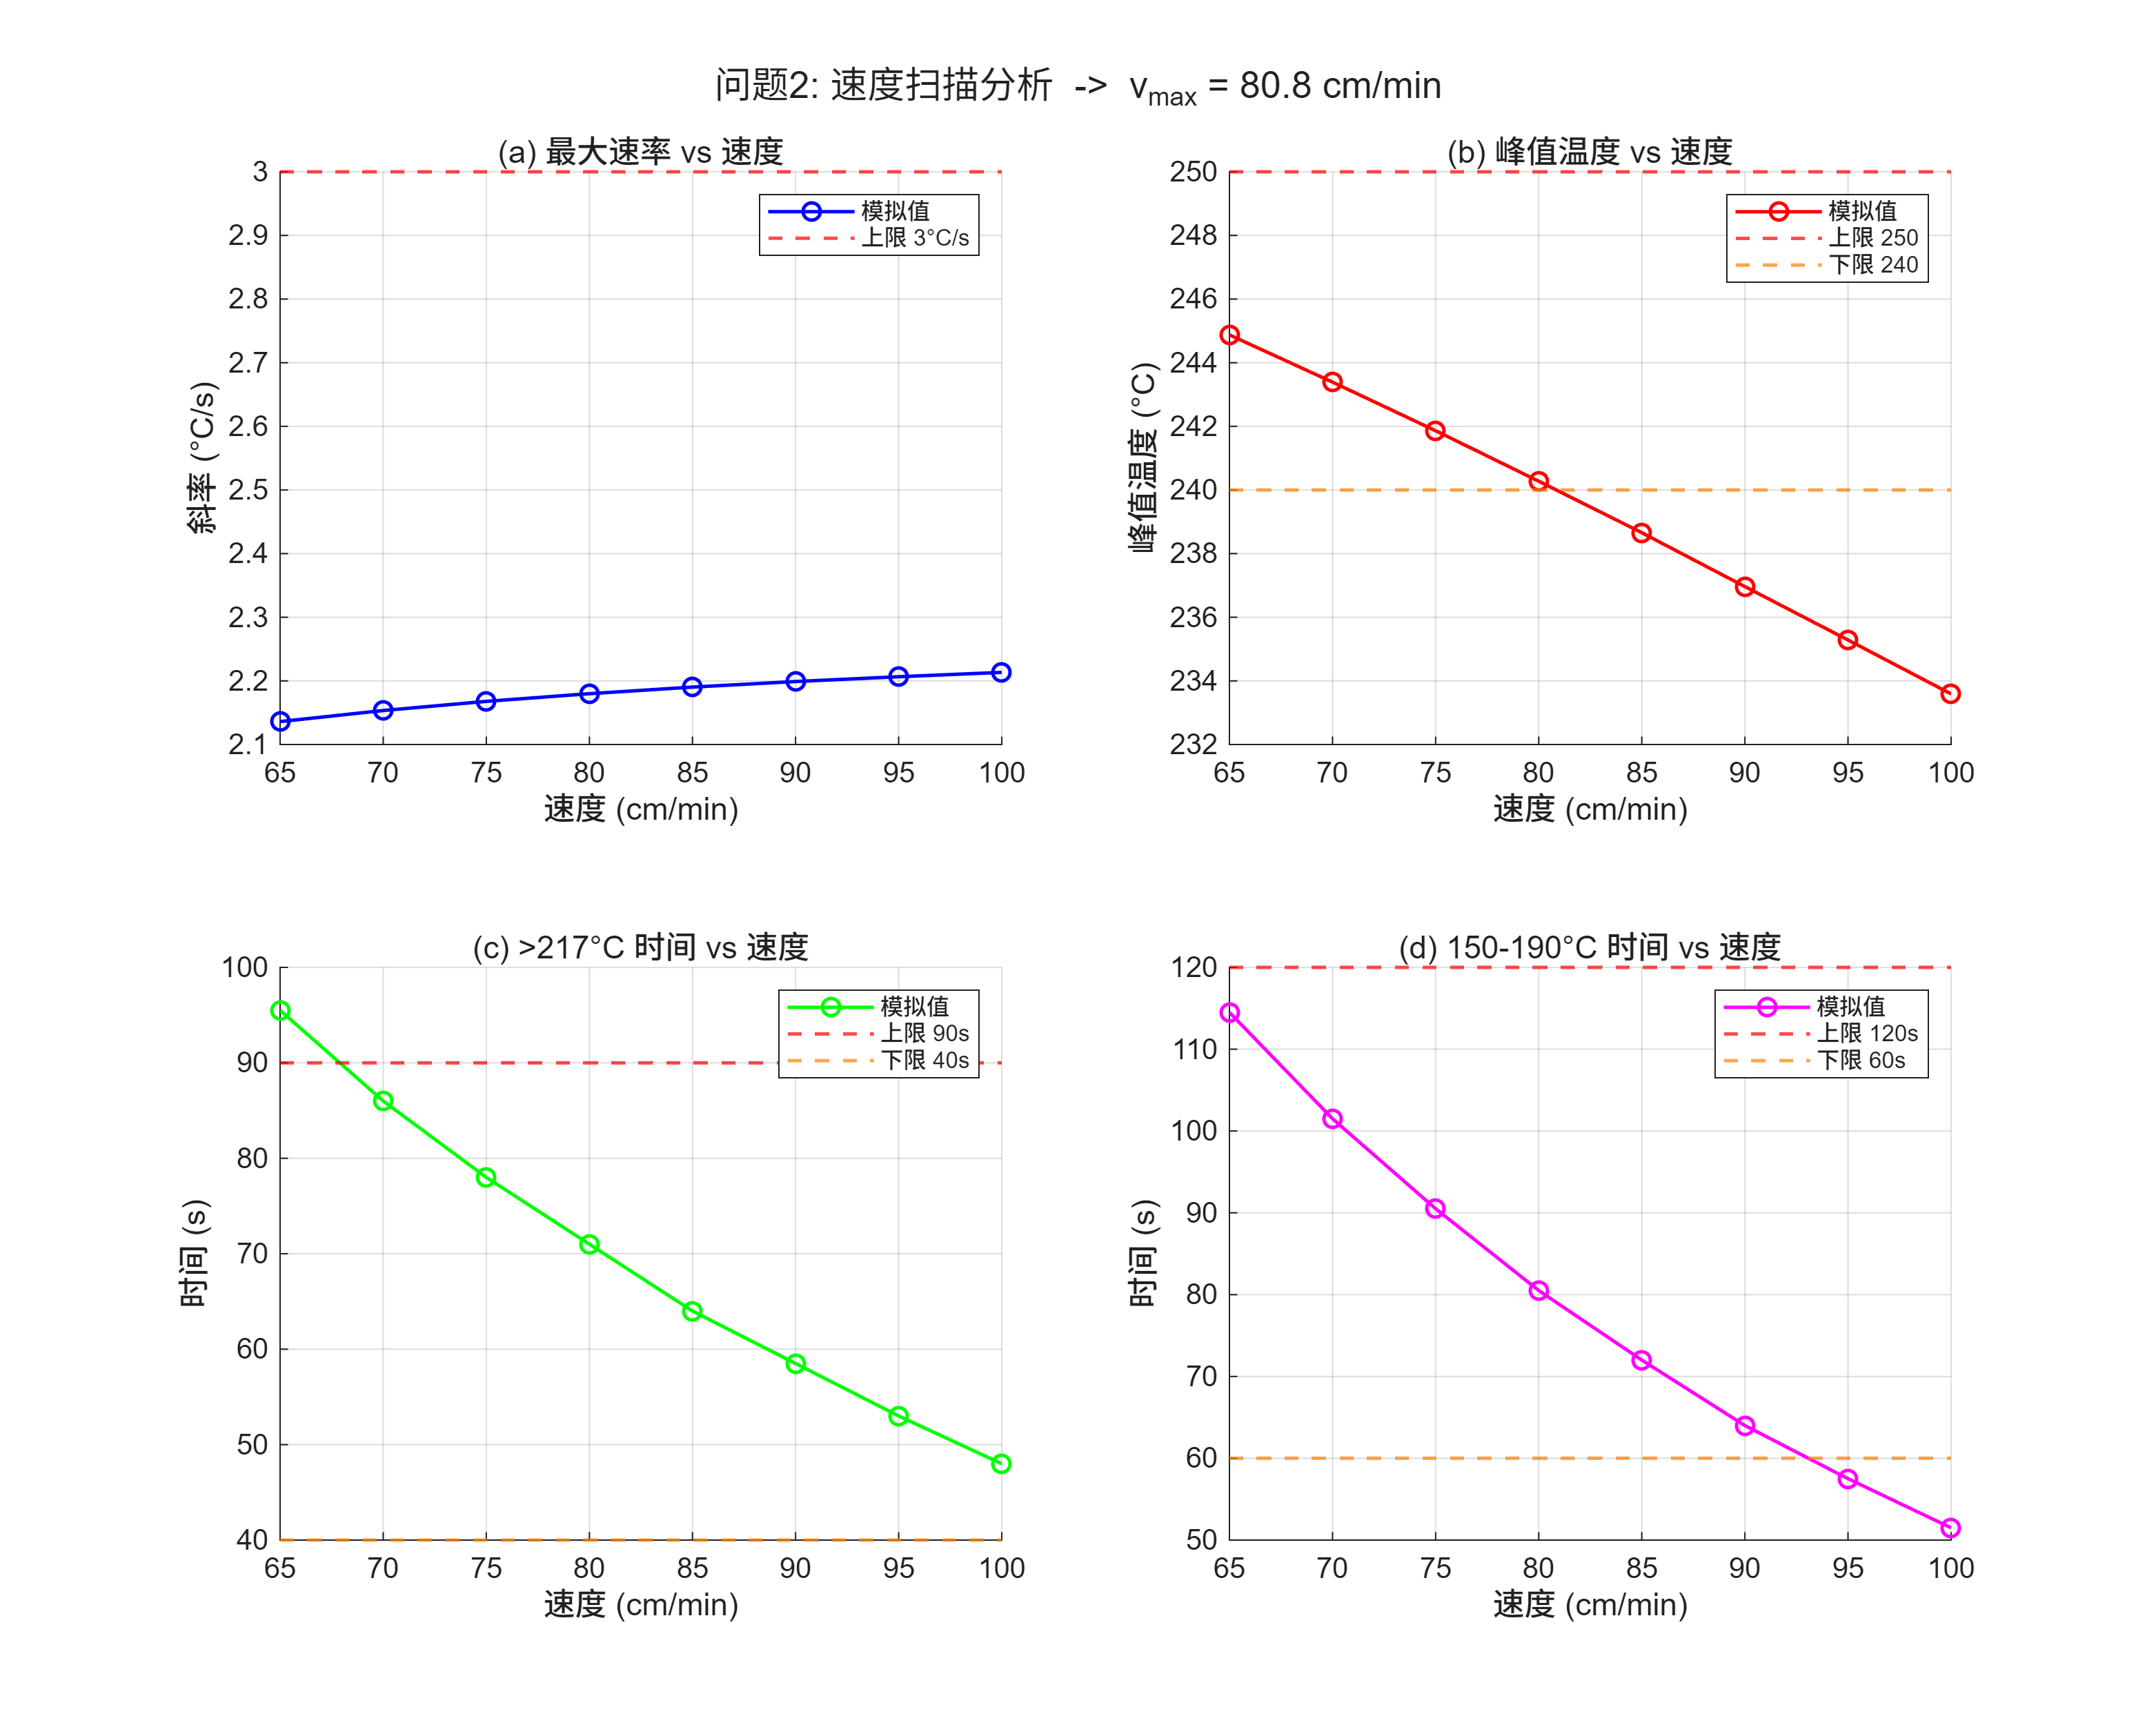
\includegraphics[width=1.1\textwidth, keepaspectratio]{../result/figures/q2_speed_analysis.png}}
\caption{问题2：速度扫描四象限分析图}
\label{fig:q2}
\end{figure}

\subsection{问题3：最小化面积}

\subsubsection{优化模型}

\begin{align}
\min_{\mathbf{x}} \quad & S(\mathbf{x}) = \int_{t_1}^{t_{peak}} \bigl(T(t;\mathbf{x}) - 217\bigr)\,\mathrm{d}t \label{eq:q3_obj} \\
\text{s.t.} \quad & 240 \leq T_{\max} \leq 250 \nonumber \\
& 60 \leq t_{150-190} \leq 120 \nonumber \\
& 40 \leq t_{>217} \leq 90 \nonumber \\
& |dT/dt|_{\max} \leq 3 \nonumber \\
& \mathbf{x} = [T_{1-5}, T_6, T_7, T_{8-9}, v]^T \nonumber \\
& 165\leq T_{1-5}\leq185,\; 185\leq T_6\leq205,\; 225\leq T_7\leq245 \nonumber \\
& 245\leq T_{8-9}\leq265,\; 65\leq v\leq100 \nonumber
\end{align}

\subsubsection{求解方法}

采用SelPSO（60粒子$\times$500迭代）在5维决策空间中搜索全局最优解\cite{ref7}。
目标函数(\ref{eq:q3_obj})中$S(\mathbf{x})$由Crank--Nicolson求解器计算，不可行解赋值为$+\infty$（硬约束惩罚）。

\subsubsection{优化结果}

最优解见表\ref{tab:q3_opt}，最优炉温曲线见图\ref{fig:q3}。

\begin{table}[H]
\centering
\caption{问题3：最优解}
\label{tab:q3_opt}
\begin{tabularx}{\textwidth}{YYY}
\toprule
\textbf{参数} & \textbf{最优值} & \textbf{搜索范围} \\
\midrule
$T_{1-5}$ (小温区1$\sim$5) & $178.1^{\circ}\mathrm{C}$ & $[165,185]$ \\
$T_6$ (小温区6)            & $194.3^{\circ}\mathrm{C}$ & $[185,205]$ \\
$T_7$ (小温区7)            & $225.9^{\circ}\mathrm{C}$ & $[225,245]$ \\
$T_{8-9}$ (小温区8$\sim$9) & $265.0^{\circ}\mathrm{C}$ & $[245,265]$ \\
$v$ (传送带速度)           & $90.90\;\mathrm{cm/min}$ & $[65,100]$ \\
\midrule
\textbf{目标最小值}         & \textbf{391.6 $^{\circ}\mathrm{C}\!\cdot\!\mathrm{s}$} & --- \\
\bottomrule
\end{tabularx}
\end{table}

\textbf{约束验证}：$T_{\max}=240.0^{\circ}\mathrm{C}$（紧约束），最大斜率$2.15\;^{\circ}\mathrm{C}/\mathrm{s}$，$150\sim190^{\circ}\mathrm{C}$时间$63.0\;\mathrm{s}$（接近下限），$>$$217^{\circ}\mathrm{C}$时间$54.5\;\mathrm{s}$。

最优解中$T_{8-9}=265.0^{\circ}\mathrm{C}$触及搜索上界，$T_{\max}=240.0^{\circ}\mathrm{C}$触及约束下界。
在物理机制上，更高的回流区温度（推动峰值温度上升）配合更快的传送带速度（缩短高温停留时间），有利于减小面积。
但$T_{\max}\geq240^{\circ}\mathrm{C}$的约束和$\pm10^{\circ}\mathrm{C}$的调整范围共同限制了进一步优化的空间。

\begin{figure}[H]
\centering
\makebox[\textwidth][c]{
\includegraphics[width=1.1\textwidth]{../result/figures/q3_optimal.png}}
\caption{问题3：最优炉温曲线（红色填充区域为超过$217^{\circ}\mathrm{C}$至峰值的面积）}
\label{fig:q3}
\end{figure}

\subsubsection{PSO收敛性分析}

图\ref{fig:pso_conv}展示了问题3（最小化面积）和问题4（最小化对称性$\sigma$）的SelPSO适应度值随迭代次数的收敛曲线。
两个优化任务均在约150代内收敛至最优值的$99\%$以上（即剩余改进空间不足总改进量的$1\%$），300代后基本稳定，500代时已充分收敛。
自然选择机制使较差粒子被持续替换，造成收敛曲线呈阶梯式下降。
问题4的收敛速度略慢于问题3（问题4在150代后改善$47\%$，而问题3为$20\%$但初始值更接近最优），
原因是对称性指标$\sigma$的梯度信息弱于面积$S$，目标函数地形更加平坦。

\begin{figure}[H]
\centering
\makebox[\textwidth][c]{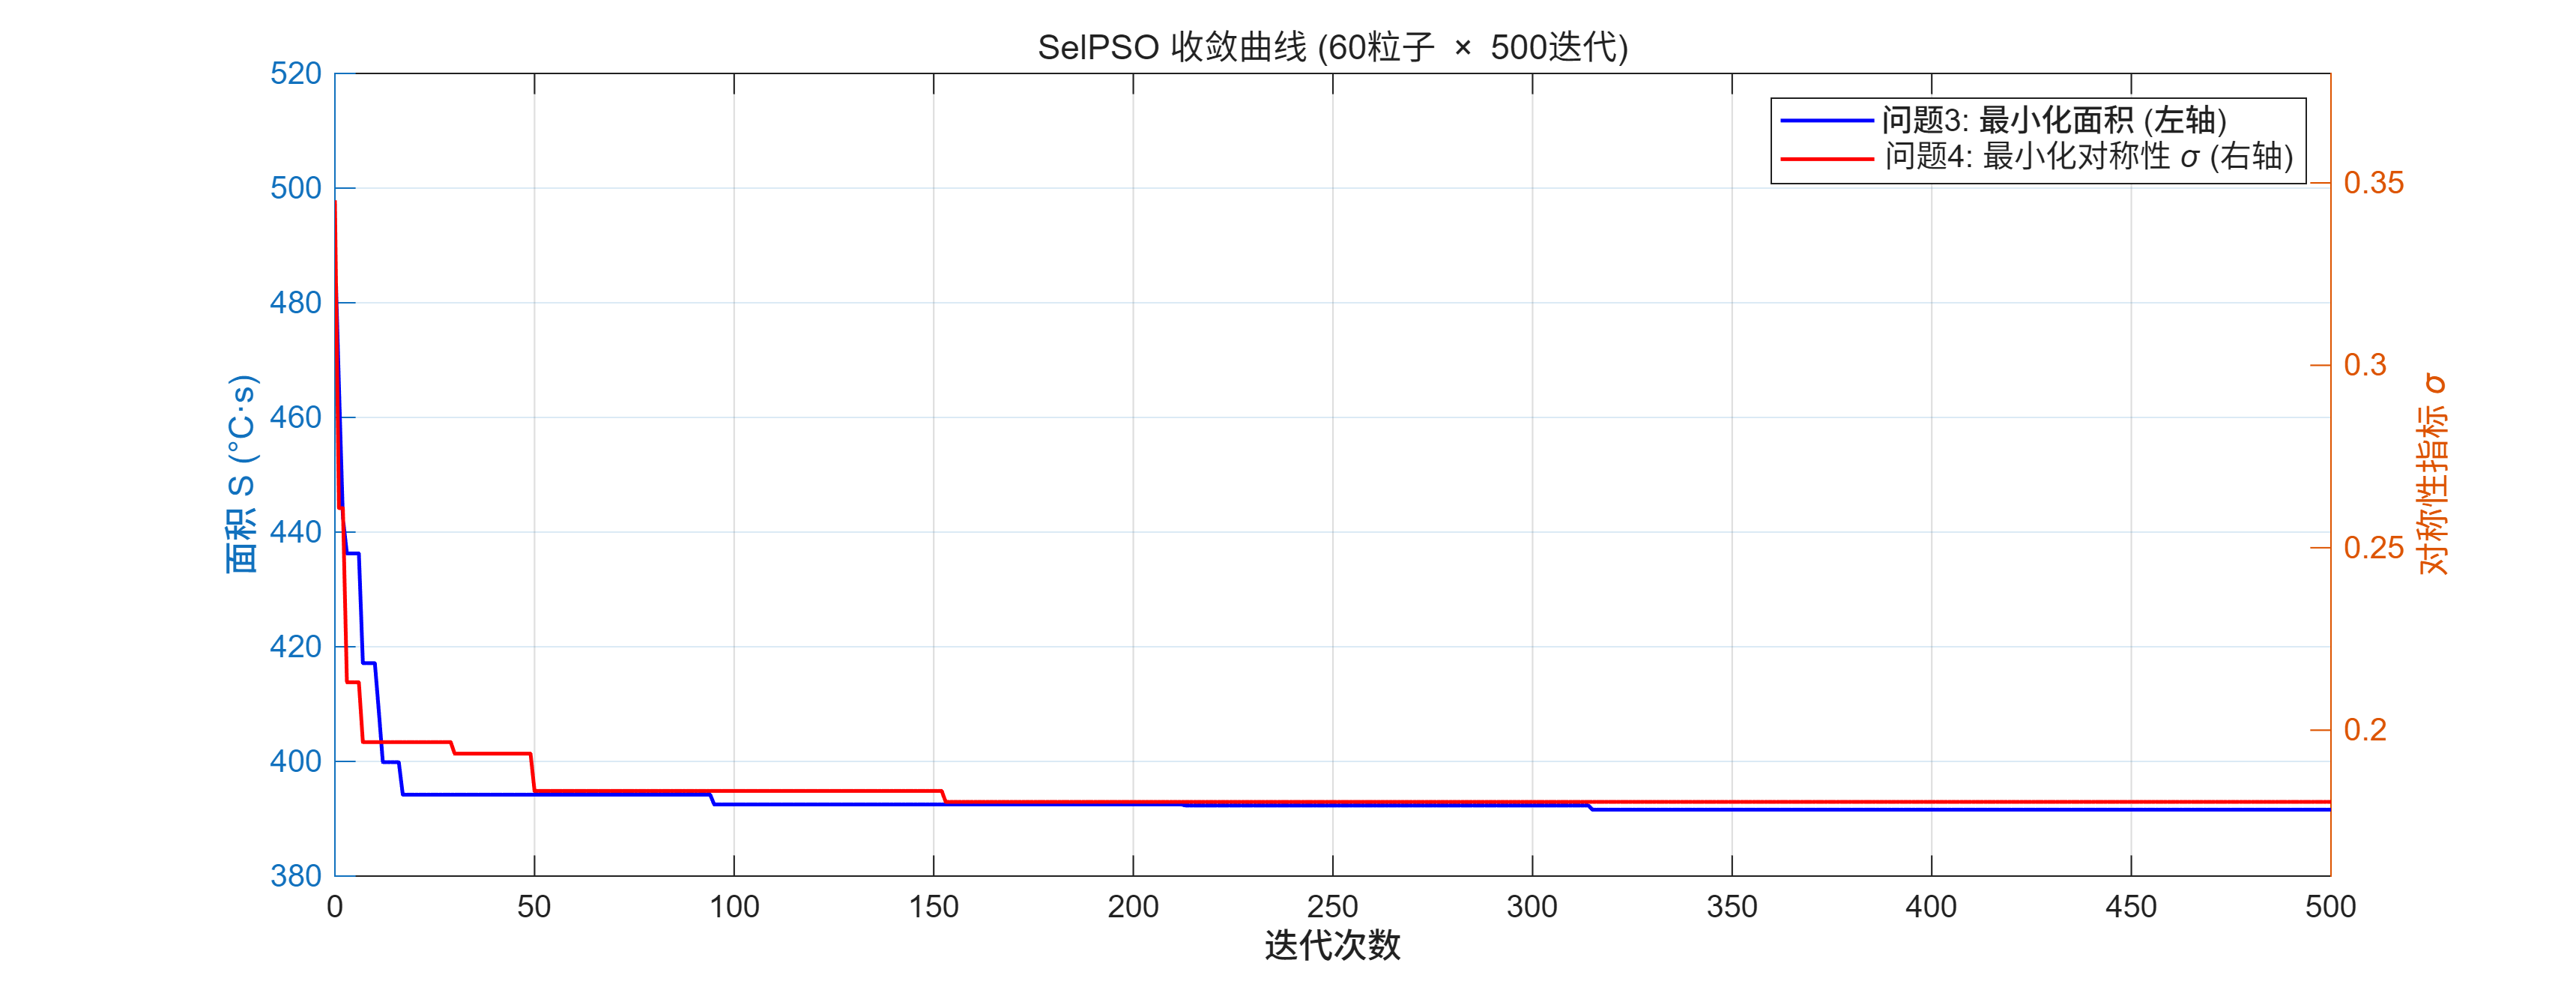
\includegraphics[width=1.1\textwidth]{../result/figures/pso_convergence.png}}
\caption{SelPSO收敛曲线（60粒子$\times$500迭代）}
\label{fig:pso_conv}
\end{figure}

\subsection{问题4：带对称性约束的优化}

\subsubsection{对称性指标}

以峰值温度对应时刻$t_{peak}$为中心线。对$T\geq217^{\circ}\mathrm{C}$的温度序列，
记峰值左侧（含峰值点）有$k$个采样点，共$n$个采样点，则左侧间隔数$n_L=k-1$，右侧间隔数$n_R=n-k$。

\textbf{面积对称性}：分别计算左右两侧超过$217^{\circ}\mathrm{C}$的梯形积分面积$A_L,A_R$，归一化差异为

\begin{equation}\label{eq:sigma1}
\sigma_1 = \frac{|A_L - A_R|}{\max(A_L, A_R)}
\end{equation}

\textbf{时间对称性}：以左右两侧采样间隔数的差异衡量，

\begin{equation}\label{eq:sigma2}
\sigma_2 = \frac{|n_L - n_R|}{\max(n_L, n_R)} = \frac{|2k - n - 1|}{\max(k-1, n-k)}
\end{equation}

\textbf{综合对称性指标}取最大值：

\begin{equation}\label{eq:sigma}
\sigma = \max(\sigma_1, \sigma_2) \in [0,1]
\end{equation}

$\sigma=0$表示完全对称，$\sigma$越接近1表示越不对称。
该指标由对称性的物理含义直接推导，同时控制了面积和时间两个维度的不对称性。

\subsubsection{优化策略与结果}

采用SelPSO直接最小化综合对称性指标$\sigma$，约束条件与问题3相同。
同时运行问题3（最小化面积）作为对比基准，结果见表\ref{tab:q4}。

\begin{table}[H]
\centering
\footnotesize
\caption{问题4：对称性优化结果对比}
\label{tab:q4}
\begin{tabularx}{\textwidth}{YYYYYYYYY}
\toprule
\textbf{方案} & \textbf{面积} & $\boldsymbol{\sigma}$ & $\boldsymbol{\sigma_1}$ & $\boldsymbol{\sigma_2}$ & $\boldsymbol{T_{1-5}}$ & $\boldsymbol{T_6}$ & $\boldsymbol{T_7}$ & $\boldsymbol{T_{8-9}}$ \\
\midrule
Q3 (最小面积)    & 391.6 & 0.1833 & ---  & ---  & 178.1 & 194.3 & 225.9 & 265.0 \\
Q4 (最小$\sigma$) & 408.8 & \textbf{0.1803} & 0.0707 & 0.1803 & 176.4 & 187.7 & 230.6 & 264.9 \\
\bottomrule
\end{tabularx}
\end{table}

问题4以面积增加$17.2\;^{\circ}\mathrm{C}\!\cdot\!\mathrm{s}$（约$4.4\%$）的代价，将对称性指标从$0.1833$改善至$0.1803$。
面积对称性$\sigma_1=0.0707$表明峰值两侧面积已高度均衡；时间对称性$\sigma_2=0.1803$是主要的不对称来源。

\begin{figure}[H]
\centering
\makebox[\textwidth][c]{
\includegraphics[width=1.1\textwidth]{../result/figures/q4_symmetric_optimal.png}}
\caption{问题4：对称最优炉温曲线（左）及对称性镜像对比分析（右）}
\label{fig:q4}
\end{figure}

% ============================================================
\section{模型检验}
% ============================================================

\subsection{拟合精度检验}

对比模拟温度与实验数据，拟合精度指标为$R^2=0.9999$，$\mathrm{RMSE}=0.62^{\circ}\mathrm{C}$，最大绝对误差$<2^{\circ}\mathrm{C}$。
残差在零线附近随机分布，无明显趋势性偏差，表明模型能够高度准确地复现实验观测。

\subsection{参数鲁棒性分析}

以问题1为基准，对核心热力学参数进行$\pm10\%$摄动测试：

\begin{table}[H]
\centering
\caption{参数敏感性分析}
\label{tab:sensitivity}
\begin{tabularx}{\textwidth}{YYY}
\toprule
\textbf{参数变化} & $\boldsymbol{\Delta T_{\max}}$ ($^{\circ}\mathrm{C}$) & $\boldsymbol{\Delta S}$ ($^{\circ}\mathrm{C}\!\cdot\!\mathrm{s}$) \\
\midrule
$a_1 +10\%$ & $+0.3$ & $+20.9$ \\
$h_1 +10\%$ & $+0.3$ & $+21.1$ \\
全部$+10\%$ & $<0.5$ & $<40$ \\
\bottomrule
\end{tabularx}
\end{table}

峰值温度对参数摄动的最大偏移$<0.5^{\circ}\mathrm{C}$，表明模型具有良好鲁棒性。

\subsection{数值格式对比}

\begin{table}[H]
\centering
\caption{Crank--Nicolson与显式Euler格式对比}
\label{tab:method_compare}
\begin{tabularx}{\textwidth}{YYY}
\toprule
\textbf{对比维度} & \textbf{显式Euler} & \textbf{Crank--Nicolson（本文）} \\
\midrule
时间精度 & $O(\Delta t)$ & $O(\Delta t^2)$ \\
稳定性   & $\Delta t < 0.01\;\mathrm{s}$ & 无条件稳定 \\
$\Delta t=0.5\;\mathrm{s}$适用性 & 不稳定 & 稳定且精度良好 \\
\bottomrule
\end{tabularx}
\end{table}

\subsection{约束满足性检验}

\begin{table}[H]
\centering
\footnotesize
\caption{四个问题最终解的制程界限验证}
\label{tab:constraints}
\begin{tabularx}{\textwidth}{YYYYYY}
\toprule
\textbf{问题} & $\boldsymbol{T_{\max}}$范围 & $\boldsymbol{|dT/dt|_{\max}}$ & $\boldsymbol{t_{150-190}}$范围 & $\boldsymbol{t_{>217}}$范围 & \textbf{结论} \\
\midrule
1 & $240.6\surd$ & $2.05\surd$ & $75.5\surd$ & $66.0\surd$ & 全部满足 \\
2 & $240.0\surd$ & $2.18\surd$ & $79.0\surd$ & $70.0\surd$ & 全部满足 \\
3 & $240.0\surd$ & $2.15\surd$ & $63.0\surd$ & $54.5\surd$ & 全部满足 \\
4 & $240.4\surd$ & $2.17\surd$ & $62.0\surd$ & $55.5\surd$ & 全部满足 \\
\bottomrule
\end{tabularx}
\end{table}

% ============================================================
\section{结果分析与讨论}
% ============================================================

\subsection{炉温曲线特征分析}

问题1的炉温曲线呈现典型的回流焊四阶段特征：
\textbf{预热阶段}（$0\sim100\;\mathrm{s}$）：温度从室温升至约$150^{\circ}\mathrm{C}$，升温速率约$1.3^{\circ}\mathrm{C}/\mathrm{s}$；
\textbf{恒温阶段}（$100\sim167\;\mathrm{s}$）：温度在$150\sim190^{\circ}\mathrm{C}$区间缓慢上升，有利于助焊剂活化；
\textbf{回流阶段}（$167\sim234\;\mathrm{s}$）：温度快速上升至峰值$240.6^{\circ}\mathrm{C}$，焊料熔化；
\textbf{冷却阶段}（$234\;\mathrm{s}$之后）：温度开始下降，焊料凝固。

\subsection{速度影响规律}

速度扫描数据揭示了清晰的单调规律：
速度每增加$5\;\mathrm{cm/min}$，峰值温度下降约$1.5^{\circ}\mathrm{C}$，$>$$217^{\circ}\mathrm{C}$时间缩短约$7\;\mathrm{s}$，温度变化斜率增加约$0.015^{\circ}\mathrm{C}/\mathrm{s}$。
速度与峰值温度的关系近似线性（$R^2>0.998$）。

\subsection{面积最小化的物理机制}

问题3的最优解将$T_{8-9}$推至$265^{\circ}\mathrm{C}$（调整范围上限），同时将速度提高到$90.90\;\mathrm{cm/min}$。
在物理上，更高的回流区温度确保峰值温度不跌破$240^{\circ}\mathrm{C}$的下限，而更快的速度缩短了高温停留时间，
两者共同作用使得超过$217^{\circ}\mathrm{C}$到峰值的面积最小化。

\subsection{对称性优化的权衡}

问题4的结果表明，面积和对称性之间存在权衡关系。
面积对称性$\sigma_1=0.0707$已接近完全对称，但时间对称性$\sigma_2=0.1803$改善空间有限。
这是因为加热和冷却的物理机制不对称（预热区换热系数$h_1=2.13\times10^{4}$远大于冷却区$h_5=1.00\times10^{3}$），
导致自然冷却过程难以与强制加热过程在时间维度上完全匹配。

\subsection{工艺建议}

基于本文的优化结果，可针对不同生产目标提出工艺建议：
追求\textbf{最高产能}时，采用问题2方案（$v=80.83\;\mathrm{cm/min}$），在保证质量的前提下最大化生产速度；
追求\textbf{最小热损伤}时，采用问题3方案（面积$=391.6\;^{\circ}\mathrm{C}\!\cdot\!\mathrm{s}$）；
追求\textbf{焊接均匀性}时，采用问题4方案（$\sigma=0.1803$）。
建议在最优参数$\pm2^{\circ}\mathrm{C}$或$\pm2\;\mathrm{cm/min}$范围内操作，所有约束仍可满足。

% ============================================================
\section{模型评价与改进}
% ============================================================

\subsection{模型优点}

\begin{enumerate}[nosep]
    \item \textbf{物理基础扎实}：基于经典的一维非稳态热传导方程，边界条件采用牛顿冷却定律，参数具有明确物理含义；
    \item \textbf{数值方法可靠}：Crank--Nicolson隐式格式具有二阶精度和无条件稳定性；
    \item \textbf{参数独立拟合}：通过SelPSO对实验数据反演获得所有热力学参数，$R^2=0.9999$验证了模型的准确性；
    \item \textbf{优化方法高效}：SelPSO全局优化结合二分搜索，在5维空间中高效求解非线性约束优化问题；
    \item \textbf{对称性指标原创}：面积与时间双维度对称性指标由对称性的物理定义直接推导，无需参考已有文献。
\end{enumerate}

\subsection{模型不足}

\begin{enumerate}[nosep]
    \item 一维传热假设忽略了焊接区域的横向传热和边缘效应；
    \item 忽略高温区（$>$$200^{\circ}\mathrm{C}$）的辐射传热贡献，可能低估实际温度；
    \item 分段常数物性假设无法描述材料性质的连续温度依赖性；
    \item PSO优化结果为随机搜索，每次运行结果可能有微小差异。
\end{enumerate}

\subsection{改进方向}

\begin{enumerate}[nosep]
    \item 建立二维或三维传热模型，考虑PCB的几何形状效应；
    \item 引入辐射传热项（Stefan--Boltzmann定律），描述对流--辐射耦合传热；
    \item 采用温度相关的变物性模型，进一步提高模拟精度；
    \item 多次PSO运行取最优结果，或采用贝叶斯优化等替代方法。
\end{enumerate}

% ============================================================
\section{结论}
% ============================================================

本文基于一维非稳态热传导理论，建立了回焊炉焊接区域温度变化的数学模型。
采用Crank--Nicolson隐式有限差分格式进行数值求解，通过SelPSO对实验数据独立拟合获得了5段分区热力学参数（$R^2=0.9999$）。
在此基础上，完成了四个问题的求解：

\textbf{问题1}：在给定参数下计算了炉温曲线，峰值温度$240.6^{\circ}\mathrm{C}$，所有制程界限均满足，温度数据已输出至result.csv。
\textbf{问题2}：通过二分搜索确定最大传送带速度为$80.83\;\mathrm{cm/min}$，限制瓶颈为峰值温度不低于$240^{\circ}\mathrm{C}$。
\textbf{问题3}：以SelPSO全局优化获得最小面积$391.6\;^{\circ}\mathrm{C}\!\cdot\!\mathrm{s}$，最优$T_{8-9}=265.0^{\circ}\mathrm{C}$，$v=90.90\;\mathrm{cm/min}$。
\textbf{问题4}：构造了面积与时间双维度对称性指标，通过直接优化$\sigma$获得对称性最优解（$\sigma=0.1803$）。

本研究的创新贡献在于：(1)~基于物理结构的分段参数策略与独立PSO拟合；(2)~Crank--Nicolson预分解快速求解技术；
(3)~SelPSO在回焊炉工艺参数优化中的应用；(4)~双维度综合对称性指标的构造与优化。

研究成果为回焊炉温度曲线的机理分析和工艺参数优化提供了可靠的理论基础和数值工具。

% ============================================================
\newpage
\begin{thebibliography}{99}

\bibitem{ref1} 杨世铭, 陶文铨. 传热学（第四版）[M]. 北京: 高等教育出版社, 2006.

\bibitem{ref5} Angeline P J. Using selection to improve particle swarm optimization[C]. Proceedings of the 1998 IEEE International Conference on Evolutionary Computation, 1998: 84-89.

\bibitem{ref4} Kennedy J, Eberhart R. Particle swarm optimization[C]. Proceedings of ICNN'95, 1995, 4: 1942-1948.

\bibitem{ref2} 陶文铨. 数值传热学（第二版）[M]. 西安: 西安交通大学出版社, 2001.

\bibitem{ref3} Crank J, Nicolson P. A practical method for numerical evaluation of solutions of partial differential equations of the heat-conduction type[J]. Mathematical Proceedings of the Cambridge Philosophical Society, 1947, 43(1): 50-67.

\bibitem{ref7} 司守奎, 孙兆亮. 数学建模算法与应用（第2版）[M]. 北京: 国防工业出版社, 2015.

\end{thebibliography}

% ============================================================
\newpage
\section*{附录：部分MATLAB核心代码}

\subsection*{Crank--Nicolson热传导求解器（solve\_heat.m）}

\begin{lstlisting}
function [T_center, T_oven, t_full] = solve_heat(F, v_cms, xm)
    L_total = 25 + 11*30.5 + 10*5 + 25;
    thickness = 0.015; dx = 1e-4; dt = 0.5; T_ambient = 25;
    total_time = L_total / v_cms;
    n = ceil(thickness/dx) + 1; m = floor(total_time/dt) + 1;
    k_center = ceil(thickness/2/dx);

    t_vec = (0:m-1)*dt; x_vec = v_cms*t_vec;
    T_oven = oven_temp(x_vec, F);

    L1 = 197.5; L2 = 233; L3 = 268.5;
    t1 = L1/v_cms; t2 = L2/v_cms; t3 = L3/v_cms;
    m1 = floor(t1/dt)+1; m2 = floor(t2/dt)+1; m3 = floor(t3/dt)+1;

    a_vals = [xm(1),xm(3),xm(5),xm(7),xm(9)];
    h_vals = [xm(2),xm(4),xm(6),xm(8),xm(10)];
    r_vals = a_vals.^2 * dt / (dx^2);

    u = zeros(n,m); u(:,1) = T_ambient;
    T_center = ones(m,1)*T_ambient;

    [C1,d1] = build_cn(n,r_vals(1),h_vals(1),m,T_oven,dx);
    for j = 1:m1-1
        u(:,j+1) = C1*u(:,j) + d1(:,j+1);
        T_center(j+1) = u(k_center,j+1);
    end
    % ... (段2-5类似，省略)
end
\end{lstlisting}

\subsection*{SelPSO优化算法核心}

\begin{lstlisting}
function [xm_best, fv_best] = sel_pso(fit, N, w, c1, c2, ...
                                      xmax, xmin, M, D, xm_data)
    Vmax = 0.2*(xmax - xmin);
    x = xmin + rand(N,D).*(xmax - xmin);
    v = Vmax.*(-1 + 2*rand(N,D));
    % 初始化个体最优与全局最优
    p = zeros(N,1); y = x;
    for i = 1:N, p(i) = fit(x(i,:), xm_data); end
    [pg, idx] = min(p); px = x(idx,:);

    for t = 1:M
        for i = 1:N
            v(i,:) = w*v(i,:) + c1*rand(1,D).*(y(i,:)-x(i,:)) ...
                               + c2*rand(1,D).*(px-x(i,:));
            v(i,:) = max(min(v(i,:), Vmax), -Vmax);
            x(i,:) = x(i,:) + v(i,:);
            if all(x(i,:)<=xmax) && all(x(i,:)>=xmin)
                f = fit(x(i,:), xm_data);
                if f < p(i), p(i)=f; y(i,:)=x(i,:); end
                if p(i) < pg, pg=p(i); px=y(i,:); end
            end
        end
        % 自然选择：较差粒子被替换
        [~,s] = sort(p); ex = round((N-1)/2);
        x(s(N-ex+1:N),:) = x(s(1:ex),:);
    end
    xm_best = px'; fv_best = pg;
end
\end{lstlisting}

\end{document}
